\documentclass[11pt]{article}

% Page Layout
\usepackage[a4paper, margin=1.1in]{geometry} % Set page size and margins

% Typography
\usepackage[T1]{fontenc} % Font encoding
\usepackage[utf8]{inputenc} % Input encoding
\usepackage{microtype} % Better typography
\usepackage{setspace} % Line spacing
\usepackage{mathptmx} % Times New Roman font for text and math
\usepackage{helvet} % Helvetica font for sans-serif
\usepackage{courier} % Courier font for monospace

\usepackage[titles]{tocloft} % For customizing the table of contents
\usepackage{hyperref} % For hyperlinks in the document
\usepackage[output-decimal-marker={,},list-final-separator={ en }]{siunitx}          % Voor handige links in je PDF. B.v. urls, referenties, etc.
\usepackage{varioref}
\usepackage[nameinlink, capitalise, noabbrev]{cleveref}
\usepackage{amsmath}
\usepackage{mathrsfs}

% Header and Footer
\usepackage{fancyhdr} % Custom headers and footers
\usepackage{fancyvrb}
\pagestyle{fancy}
\fancyhf{}
\fancyhead[L]{\leftmark} % Chapter name on the left
\fancyhead[R]{\thepage} % Page number on the right
\fancyfoot[C]{}

% Section Titles
\usepackage{titlesec} % Customize section titles
\titleformat{\chapter}[hang]{\normalfont\huge\bfseries}{\thechapter.}{20pt}{\Huge\bfseries}

% Customize the table of contents appearance
\renewcommand{\cftchapfont}{\normalfont\bfseries}
\renewcommand{\cftsecfont}{\normalfont}
\renewcommand{\cftsubsecfont}{\normalfont}
\renewcommand{\cftchappagefont}{\normalfont\bfseries}
\renewcommand{\cftsecpagefont}{\normalfont}
\renewcommand{\cftsubsecpagefont}{\normalfont}
\renewcommand{\cftchapleader}{\cftdotfill{\cftdotsep}} % Dotted lines between section titles and page numbers

% Figures and Tables
\usepackage{graphicx} % Including images
\usepackage{subcaption} % Subfigures
\usepackage{float} % Improved float placement
\usepackage{booktabs} % Professional-looking tables
\usepackage{longtable} % Tables spanning multiple pages
\usepackage{array} % Extended array and tabular features

% References and Bibliography

\hypersetup{
colorlinks=true,
linkcolor=black,
filecolor=magenta,
urlcolor=cyan,
citecolor=blue,
pdftitle={Your Thesis Title},
pdfpagemode=FullScreen,
}


% Miscellaneous
\usepackage{amsmath, amssymb} % Mathematical symbols and fonts
\usepackage{enumitem} % Customized lists
\usepackage{csquotes}
% Context-sensitive quotation facilities
\usepackage{cleveref}

\linespread{1.2}              
\author{Caspar van Eck, 12652857} % vul in
\title{Machine Learning Based Event Classification in Fully Hadronic Vector Boson Scattering Events at the LHC} % Vul in.
\date{\today}


\begin{document}

\begin{titlepage}

\begin{figure}
\centering  
\includegraphics[width=80mm]{figures/Nikhef.png}\\ 
\vspace{-0ex}
\end{figure}


\maketitle
\thispagestyle{empty} 

\vfill

\begin{table}[h]
\label{tab:credits}
\begin{tabular}{l l}
\textsc{Course}  & Master thesis (60EC) at Nikhef, conducted between 01-09-2025 and 31-06-2026\\ % Vul in
\textsc{Universities}  & Universiteit van Amsterdam \& Vrije Universiteit Amsterdam \\ % Vul in
\textsc{Faculty} & Faculteit der Natuurwetenschappen, Wiskunde en Informatica \\ % Vul in
\textsc{Supervisor} & dr. Flavia de Almeida Dias \\ % Aanpassen
\textsc{Daily Supervisors} & Samuel Jankových MSc.\\ % Vul in
\textsc{Examiner} & dr. Clara Nellist\\
\end{tabular}
\vspace{3ex}
\end{table}

\begin{figure}
\centering  
\includegraphics[width=150mm]{figures/logo-combi-vu-uva-nl.png}\\   % UvA logo
\vspace{-13ex}
\end{figure}

\end{titlepage}

\clearpage
\pagenumbering{roman} % Use roman page numbering for TOC, LOF, LOT
\tableofcontents
\clearpage
\pagenumbering{arabic} % Switch to arabic numbering for main content

\setcounter{page}{2}    

\suppressfloats[t]      

\newpage
\section{Introduction}
The effort to understand the fundamental structure of matter has driven scientific progress since the start of civilization. Ideas about the composition of matter have grown into the quantitative field of particle physics. Modern particle physics combines quantum field theory with large scale accelerator experiments capable of probing interactions beyond those accessible in any other scientific context. At the centre of this experimental program is CERN, where high-energy proton beams are brought into collision to study rare and energetic processes.

\chapter{The Standard Model}
The Standard Model, illustrated in figure \ref{fig:SM}, is a quantum field theory describing the known elementary particles and the strong, weak, and electromagnetic interactions. Its structure is determined by the gauge symmetry
\begin{equation}
SU(3)_{C}\times SU(2)_{L}\times U(1)_{Y},
\end{equation}
which contrains the interaction terms and fixes the form  of the Lagrangian. The strong interaction is governed by the non-Abelian colour group $SU(3)_{C}$, while the electroweak theory unifies the weak and electromagnetic forces through the groups $SU(2)_{L}$ and $U(1)_{Y}$.
\begin{figure}[h]
    \centering
    \includegraphics[scale=0.15]{figures/Standard.png}
    \caption{The Standard Model of particle physics. Showing the quarks (purple), leptons (green), gauge bosons (red) and the Higgs boson (yellow).}
    \label{fig:SM}
\end{figure}

\section{Vector Boson Scattering}
\section{Beyond the Standard Model}
\section{Effective Field Theory}
\subsection{Standard Model Effective Field Theory}
\subsection{Anomalous Quartic Gauge Couplings}

\chapter{Recurrent Neural Networks}
\label{chap:ml}
Recurrent neural networks (RNN) are an efficient framework for processing collider inputs that naturally form sequences of variable length. In this analysis an RNN architecture is used to classify fully hadronic VBS events using per-constituent jet information.
\section{VBF-RNN}
The input to the classifier is constructed from the constituents of the two large-\(R\) jets. Constituents are ordered by decreasing transverse momentum and truncated or padded to a fixed sequence length \(T\). For each constituent a set of low-level observables is used, typically $(p_{T},\;\eta,\;\phi,\;E)\,$, as seen in figure~\ref{fig:vbfrnn}

Jets with fewer than \(T\) constituents are padded with masked entries, and the masking is propagated through the recurrent layers to ensure that padded elements do not contribute to the hidden-state evolution.
\begin{figure}[h]
    \centering
    \includegraphics[scale=0.4]{figures/VBFRNN.png}
    \caption{Illustration of the VBF-RNN architecture.}
    \label{fig:vbfrnn}
\end{figure}
\section{Testing}

\chapter{The ATLAS Detector}
\label{chap:atlas}
The A Toroidal LHC ApparatuS (ATLAS) is the largest general purpose detector at the LHC.  It is designed to record and reconstruct the products of proton proton collisions over a broad range of energies and final state topologies. The detector combines tracking, calorimetry, and muon detection systems in order to provide precise measurements of charged particle trajectories, particle energies, and event level observables. 

ATLAS is built in a cylindrical geometry around the beam axis, with subdetectors arranged in concentric layers. The coordinate system is defined with its origin at the nominal interaction point. The $z$ axis is aligned with the beam direction, the $x$ axis points from the interaction point toward the centre of the LHC ring, and the $y$ axis points upward. In the plane transverse to the beam, particle directions are described by the azimuthal angle $\phi$. The polar angle $\theta$ with respect to the beam axis is commonly expressed in terms of pseudorapidity $\eta = -\ln\tan(\theta/2)$

\begin{figure}[H]
    \centering
    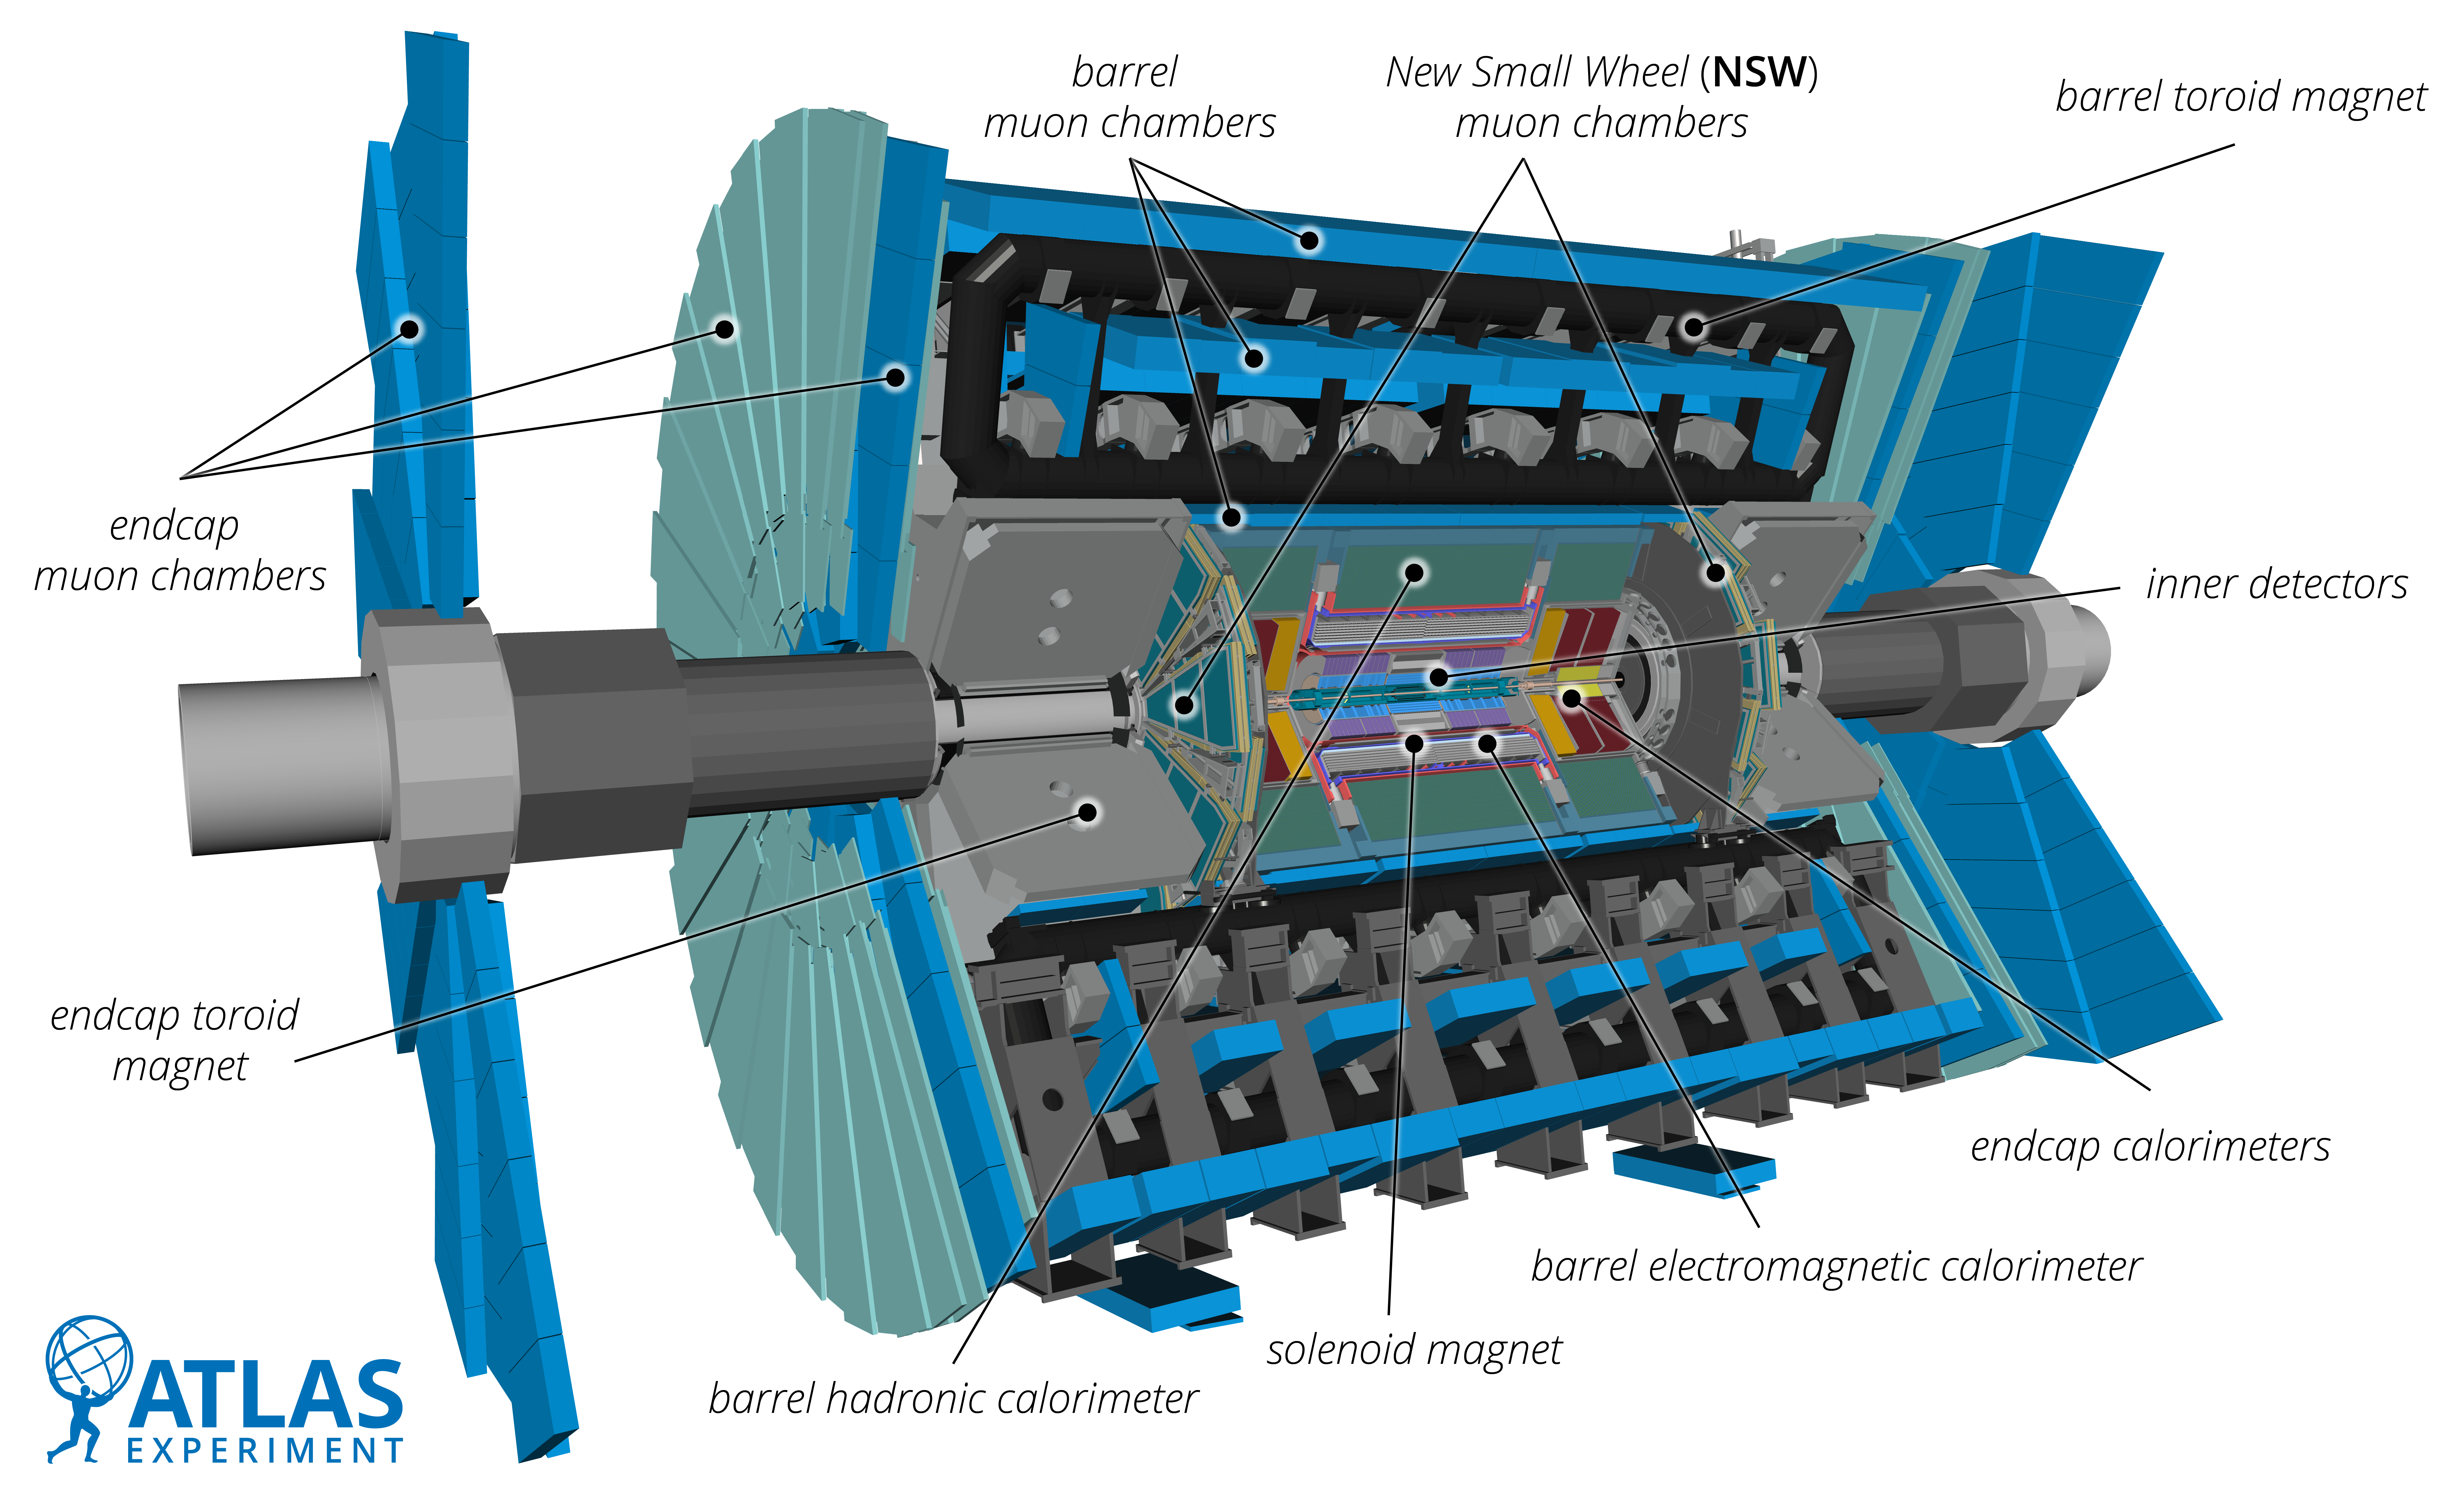
\includegraphics[width=0.95\textwidth]{figures/Detector.png}
    \caption{Schematic view of the ATLAS detector.}
    \label{fig:atlas_detector}
\end{figure}

\chapter{Methods}
\label{chap:methods}
\section{Signal vs. Background Classification}

\input{results}
\input{conclusion}
\input{discussion}
\input{outlook}


\bibliographystyle{science}
\bibliography{bibliography.bib}

\end{document}
